% !TEX program  = xelatex

\documentclass{article}
\usepackage{ctex}
\usepackage[ruled,vlined,linesnumbered]{algorithm2e}
\usepackage{algpseudocode}
\usepackage{amsmath}
\usepackage{amsthm}
\usepackage{graphicx}
\usepackage{subfigure}
\usepackage{float}
\usepackage{amsmath }
\usepackage{amsfonts }
\usepackage{pdfpages}
\usepackage{epsfig}
\usepackage{graphicx}
\usepackage{arydshln}
\usepackage{verbatim}
\usepackage{subfigure}
\usepackage{enumerate}
\usepackage{rotating}
\usepackage{threeparttable}
\usepackage{caption}
\usepackage{tikz}
\usepackage{epsfig}
\usepackage{cite}
\usepackage{geometry}
\usepackage{listings}
\usepackage{fontspec}
\newfontfamily\codefont{times.ttf}
\setCJKmainfont{SourceHanSerifCN-Regular-1.otf}
\lstdefinestyle{mystyle}{
	frame=tb,
	aboveskip=3mm,
	belowskip=3mm,
	showstringspaces=false,
	columns=flexible,
	framerule=1pt,
	rulecolor=\color{gray!35},
	backgroundcolor=\color{gray!5},
	basicstyle={\small\ttfamily},
	numbers=left,        % 显示行号
	numberstyle=\tiny\color{gray},
	numbersep=5pt,
	keywordstyle=\color{blue},
	commentstyle=\color{green!50!black},
	stringstyle=\color{red!80!black},
	breaklines=true,
	breakatwhitespace=true,
	tabsize=3,
	% 添加新的样式定义
	identifierstyle=\color{black},    % 变量名称颜色
	emphstyle=\color{purple},        % 函数名称颜色
	morecomment=[l][\color{magenta}]{\#}, % 行内注释颜色
}
\geometry{a4paper, top=2.4cm, bottom=2.4cm, left=3cm, right=3cm}
\usepackage[colorlinks,linkcolor=black]{hyperref}
\linespread{1}
\begin{document}
	\title{AU3303 机器人学~~实验报告}
	\author{王凯灵 521030910356 F2103801}
	\date{2023.10.8}
	\maketitle
	\section*{1}
	按照理论课给出的DH参数推导方法，使用modeified模式传入DH参数。代码如下：
	\begin{lstlisting}[language=MATLAB, style=mystyle]
	theta = [0, 0, 0, 0, 0, 0];
	d = [0, 0, 20, 100, 0, 0];
	a = [0, 0, 100, 10, 0, 0];
	alpha = [0, -pi/2, 0, -pi/2, pi/2, -pi/2];
	
	L1 = Link([theta(1), d(1), a(1), alpha(1)], 'modified');
	L2 = Link([theta(2), d(2), a(2), alpha(2)], 'modified');
	L3 = Link([theta(3), d(3), a(3), alpha(3)], 'modified');
	L4 = Link([theta(4), d(4), a(4), alpha(4)], 'modified');
	L5 = Link([theta(5), d(5), a(5), alpha(5)], 'modified');
	L6 = Link([theta(6), d(6), a(6), alpha(6)], 'modified');
	p560 = SerialLink([L1, L2, L3, L4, L5, L6], 'name', 'PUMA560');
	\end{lstlisting}

	\begin{figure}[ht!]
		\centering
		\begin{minipage}{0.45\textwidth}
			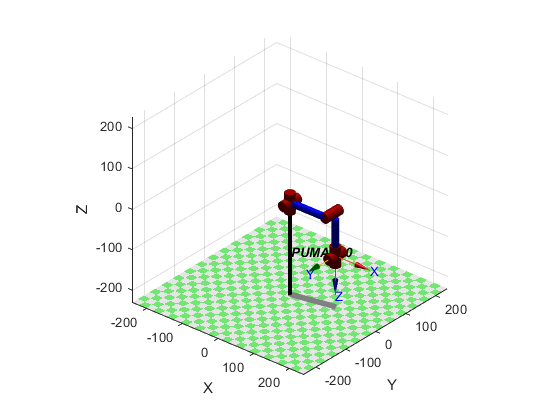
\includegraphics[width=\linewidth]{../imgs/p560}
			\caption{绘制的PUMA560}
			\label{puma}
		\end{minipage}
		\hfill
		\begin{minipage}{0.45\textwidth}
			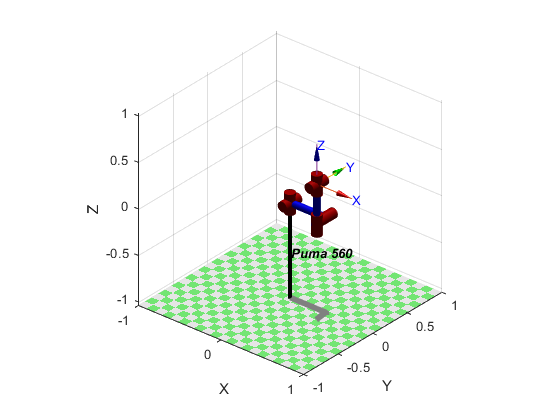
\includegraphics[width=\linewidth]{../imgs/mdl_p560}
			\caption{预定义的PUMA560}
			\label{mdl_puma}
		\end{minipage}
	\end{figure}

	绘制出的PUMA560机械臂如图\ref{puma}所示，而工具箱预定义的puma560如图\ref{mdl_puma}所示，两者存在明显不同。观察DH参数设置并分析：首先，标准DH与改进DH参数正方向相反，故预定义的末端朝上。两种定义方法坐标定义不同，造成关节可视化位置的差异，尤其是第四个关节消失。经过检验，第四个关节正确定义，只是并没有显示出来。之后的任务中，将使用自定义的PUMA560。
	
	通过随机采样10000组关节参数，使用正运动学得到执行器坐标，代码如下：
	\begin{lstlisting}[language=MATLAB, style=mystyle]
	total = 10000;
	sampled_poses = zeros(total, 4, 4);
	param_list = zeros(total, 6);
	
	for sample = 1:total
		q = ([rand(), rand(), rand(), rand(), rand(), rand()] - 0.5) * 2 * pi;
		param_list(sample, :) = q;
		sampled_poses(sample, :, :) = p560.fkine(q);
	end
	% Visualization code is lengthy; please refer to the raw code.
	\end{lstlisting}

	可见在该机械臂长度设置下，工作空间是一个球体，除去关节1所在的柱形区域（如图\ref{c}）。图\ref{cup}显示了上视图，中心区域不可到达。从概率的角度，还能看出在靠近工作边缘的部分，采样点较为稀疏，因为只有更小的关节参数范围可以到这些位置。
	\begin{figure}[ht!]
		\centering
		\begin{minipage}{0.45\textwidth}
			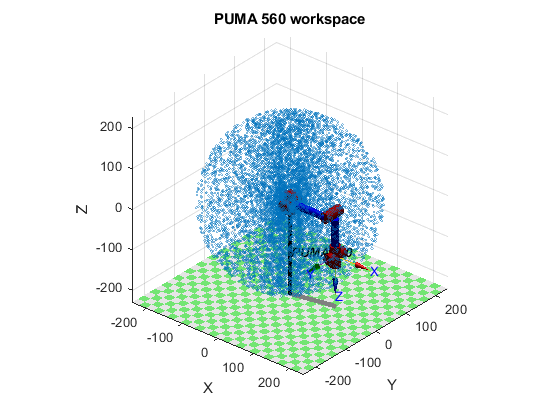
\includegraphics[width=\linewidth]{../imgs/circle}
			\caption{完整的工作空间}
			\label{c}
		\end{minipage}
		\hfill
		\begin{minipage}{0.45\textwidth}
			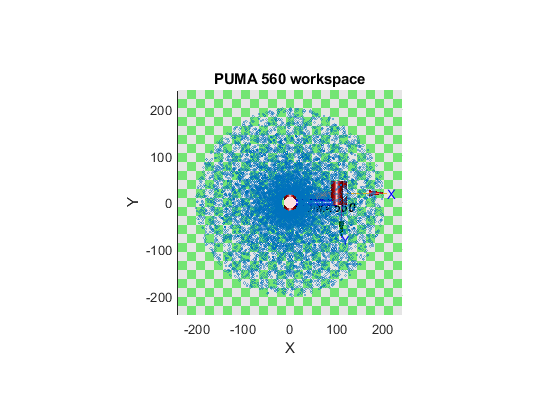
\includegraphics[width=\linewidth]{../imgs/circle_up}
			\caption{工作空间上视图}
			\label{cup}
		\end{minipage}
	\end{figure}

	在$-90<q<90$的范围内进行采样，得到的三视图如图\ref{h1}-\ref{h4}所示.
	\begin{figure}[ht!]
		\centering
		\begin{minipage}{0.45\textwidth}
			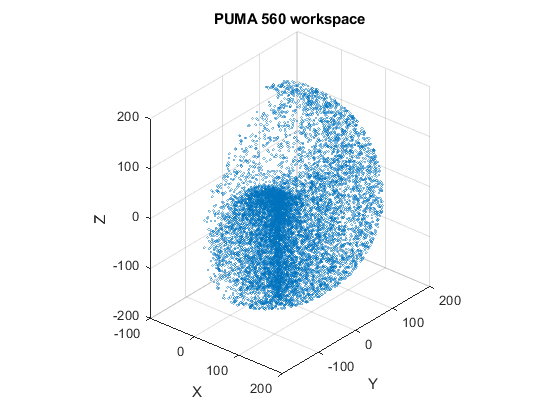
\includegraphics[width=\linewidth]{../imgs/half}
			\caption{90工作空间}
			\label{h1}
		\end{minipage}
		\hfill
		\begin{minipage}{0.45\textwidth}
			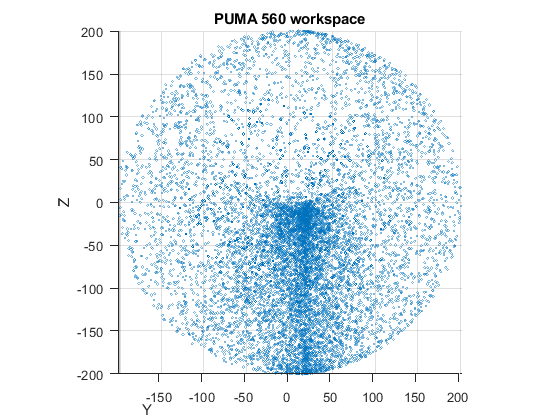
\includegraphics[width=\linewidth]{../imgs/half1}
			\caption{90工作空间前视图}
			\label{h2}
		\end{minipage}
	\end{figure}	
	\begin{figure}[ht!]
		\centering
		\begin{minipage}{0.45\textwidth}
			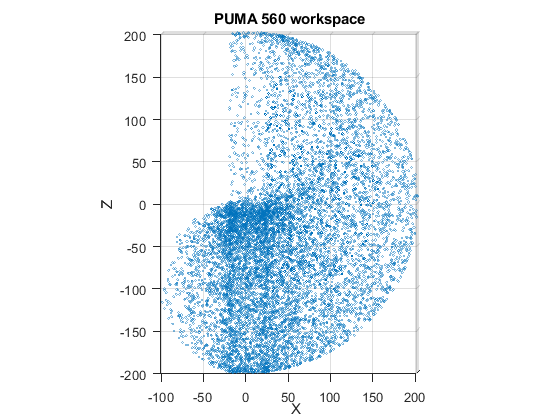
\includegraphics[width=\linewidth]{../imgs/half2}
			\caption{90工作空间左视图}
			\label{h3}
		\end{minipage}
		\hfill
		\begin{minipage}{0.45\textwidth}
			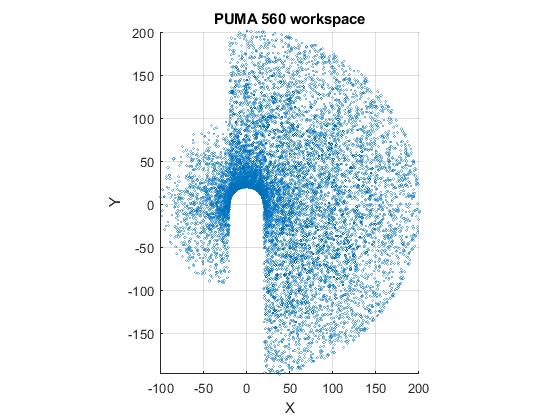
\includegraphics[width=\linewidth]{../imgs/half3}
			\caption{90工作空间上视图}
			\label{h4}
		\end{minipage}
	\end{figure}
	\section*{2}
	首先立即意识到障碍物经过原点，机械臂的基座标（即第一个关节）不能放置在原点。观察发现目标点起点在障碍物下半部分位置，如果将机械臂置于障碍物上方，会够不着。于是将机械臂基座标沿z复方向移动75。绘制机械臂与障碍物如图\ref{b}。
	
	\begin{figure}[ht!]
		\centering
		\begin{minipage}{0.45\textwidth}
			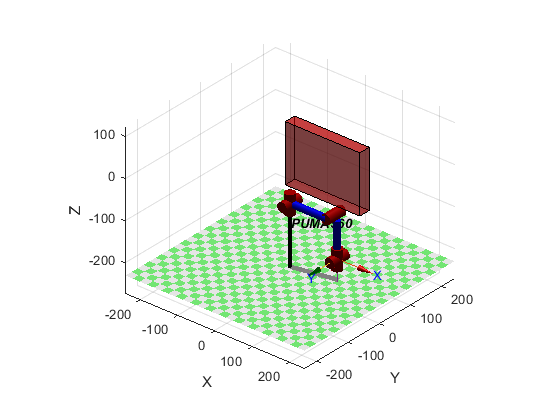
\includegraphics[width=\linewidth]{../imgs/blocked}
			\caption{机械臂与障碍物}
			\label{b}
		\end{minipage}
		\hfill
		\begin{minipage}{0.45\textwidth}
			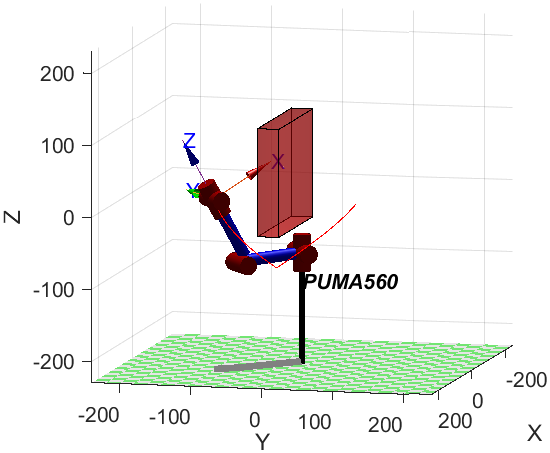
\includegraphics[width=\linewidth]{../imgs/movement}
			\caption{机械臂移动轨迹}
			\label{bt}
		\end{minipage}
	\end{figure}

	起点与终点坐标连线经过障碍物，关于障碍物对称。于是，只需要将路径改为从障碍物下方经过，即添加中点\texttt{[150, 0, -75]}即可。然而，此时机械臂地第三个关节向上突起，会与障碍物相撞。进一步调整参数，使得机械臂第三个关节初状态为\texttt{pi}，即向下弯折。在运动过程中，各关节角度变化如图\ref{ja}所示。
	\begin{figure}[ht!]
		\centering
		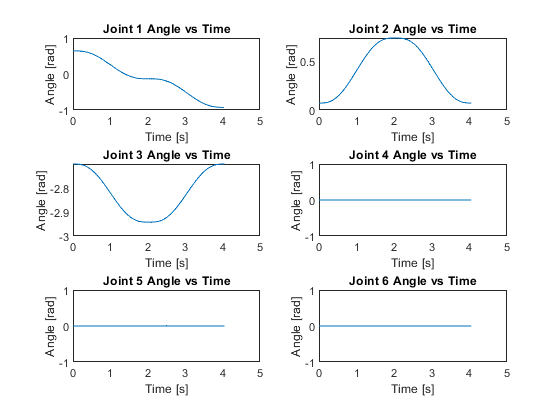
\includegraphics[width=0.8\linewidth]{../imgs/ja}
		\caption{角度变化曲线}
		\label{ja}
	\end{figure}

	路径计算相关代码如下：
	\begin{lstlisting}[language=MATLAB, style=mystyle]
	Tstart = transl(100, 100, 10);
	Tend = transl(100, -100, 10);
	
	Tmid = transl(150, 0, -75);
	
	qstart = p560.ikine(Tstart, 'q0', [0 0 pi 0 0 0], 'mask', [1 1 1 0 0 0]);
	qmid = p560.ikine(Tmid, 'q0', qstart, 'mask', [1 1 1 0 0 0]);
	qend = p560.ikine(Tend, 'q0', qmid, 'mask', [1 1 1 0 0 0]);
	
	t = 0:0.05:2;
	
	[Q1, Qd1, Qdd1] = jtraj(qstart, qmid, t);
	[Q2, Qd2, Qdd2] = jtraj(qmid, qend, t);
	patch('Vertices', vertices, 'Faces', faces, 'FaceColor', 'r', 'FaceAlpha', 0.5);
	Q = [Q1; Q2];
	p560.plot(Q, 'trail', 'r-');
	\end{lstlisting}

	所有次要代码、绘图代码都在源文件中。机械臂运动动画可在\href{https://loping151.top/images/p560\_animation.gif}{轨迹动画}在线观看，仅保证本学期内有效。

\end{document}